\title{EE5311 -- Assignment 3}
\author{Joyen Benitto}
\date{\today}
\maketitle

\section{Problem 1: Static CMOS Inverter -- Transient Characteristics}

\subsection*{Device Parameters}

The following long-channel/velocity-saturation parameters (sky130, 1.8 V
process) are used throughout this problem, as in Assignments 1 and 2:

\begin{itemize}
  \item nMOS: $V_{Tn} = 0.7$ V, $\mu_n = 0.025\ \text{m}^2/\text{Vs}$, $C_{oxn} =
  8.34\ \text{fF}/\mu\text{m}^2$, $v_{satn} = 8\times10^4$ m/s
  \item pMOS: $|V_{Tp}| = 0.7$ V, $\mu_p = 0.009\ \text{m}^2/\text{Vs}$, $C_{oxp}
  = 8.16\ \text{fF}/\mu\text{m}^2$, $v_{satp} = 3\times10^4$ m/s
\end{itemize}

\subsection*{Circuit}

A static CMOS inverter ($L_n=L_p=0.15\ \mu\text{m}$, $W_n=0.42\ \mu\text{m}$
fixed, $W_p$ swept) drives an identical inverter (fan-out of 1). \texttt{Vin}
is a PULSE source between $0$ and $V_{DD}$ with $5$~ps rise/fall time and a
$250$~ps pulse width, implemented in \texttt{inverter.sch}/\texttt{.spice}
(the shared inverter subcircuit, parametrized by \texttt{width\_p}) and
instantiated twice in each \texttt{assign1*.spice}.

\paragraph{Analytical delay model.} As in Assignments 1--2, the drain current
uses the velocity-saturation model with $L\xi_c = v_{sat}L/\mu$. Approximating
the discharge/charge current as constant at its value near the switching point
(full gate overdrive $V_{gt}=V_{DD}-V_T$) gives the averaged-current estimate
\[
I_{av} = \frac{K'(W/L)\,(V_{DD}-V_T)^2}{1 + (V_{DD}-V_T)/(L\xi_c)},
\qquad
t_p = \frac{C_{tot}\,(V_{DD}/2)}{I_{av}},
\]
applied separately to the nMOS pull-down ($t_{pHL}$, using $K_n'(W/L)_n$,
$L\xi_{c,n}$) and pMOS pull-up ($t_{pLH}$, using $K_p'(W/L)_p$,
$L\xi_{c,p}$), with $t_p=(t_{pHL}+t_{pLH})/2$. $C_{tot}\approx3.8$~fF is taken
as the lumped self+fan-out capacitance of the FO1 stage (the same value used
in \texttt{assign1b.spice}/\texttt{assign1c.spice}).

Using $k_n'=\mu_nC_{oxn}\approx208.5\ \mu\text{A/V}^2$, $k_p'=\mu_pC_{oxp}
\approx73.44\ \mu\text{A/V}^2$ (as in Assignments 1--2) and $(W/L)_n=2.8$
fixed, $K_n'(W/L)_n = 583.8\ \mu\text{A/V}^2$. The raw critical-field lengths
from Assignment 1's model are $L_n\xi_{c,n}=v_{satn}L_n/\mu_n=0.48$~V and
$L_p\xi_{c,p}=v_{satp}L_p/\mu_p=0.50$~V; the accompanying \texttt{.control}
blocks below instead use $2\times$ these values ($0.96$~V, $1.0$~V) for the
in-line analytical curve. This factor-of-2 should be revisited once simulated
data is available to calibrate against -- the tables in this section use the
script's own constants ($0.96$~V/$1.0$~V) so the hand calculation matches
what \texttt{assign1b.spice}/\texttt{assign1c.spice} will plot.

\subsection{Part (a): Delay vs.\ $W_p$ ($0.42$, $0.84$, $1.26\ \mu\text{m}$) at $V_{DD}=1.8$~V}

\subsubsection{Calculation}

With $V_{DD}=1.8$~V fixed, $t_{pHL}$ (set entirely by the fixed nMOS) is the
same for all three cases; only $t_{pLH}$ (pMOS pull-up) changes with $W_p$.
Table~\ref{tab:1a-analytical} applies the model above, holding $C_{tot}=3.8$~fF
fixed across all three $W_p$ (i.e.\ ignoring the extra self/fan-out
capacitance a larger $W_p$ itself adds -- see Discussion).

\begin{table}[h]
  \centering
  \begin{tabular}{|c|c|c|c|c|}
    \hline
    $W_p$ ($\mu$m) & $(W/L)_p$ & $t_{pHL}$ (ps) & $t_{pLH}$ (ps) & $t_p$ (ps) \\
    \hline
    0.42 & 2.8 & 10.39 & 28.87 & 19.63 \\
    0.84 & 5.6 & 10.39 & 14.44 & 12.41 \\
    1.26 & 8.4 & 10.39 & 9.62  & 10.01 \\
    \hline
  \end{tabular}
  \caption{Analytical $t_p$ vs.\ $W_p$ at $V_{DD}=1.8$~V, fixed $C_{tot}=3.8$~fF
  (averaged-current model above).}
  \label{tab:1a-analytical}
\end{table}

This idealized (fixed-$C_{tot}$) model predicts delay falling monotonically as
$W_p$ increases, with the minimum at the largest swept width ($1.26\
\mu\text{m}$). In practice $C_{tot}$ itself grows with $W_p$ (larger pMOS
drain/gate capacitance loads both the driving stage and its identical FO1
load), so the true minimum measured in simulation can sit at a smaller $W_p$
than this simplified estimate suggests -- \texttt{assign1b.spice} and
\texttt{assign1c.spice} both hard-code \texttt{width\_p = 0.84}, implying
$W_p=0.84\ \mu\text{m}$ (not $1.26$) was found to minimize delay once this
loading is accounted for in simulation. This is confirmed by simulation below
(Table~\ref{tab:1a-sim}): $W_p=0.84\ \mu\text{m}$ does give the minimum
measured delay, not $1.26\ \mu\text{m}$.

\subsubsection{Schematic}

\begin{figure}[h]
  \centering
  
\includegraphics[width=0.9\textwidth]{figures/1a_schematic.png}
  \caption{Static CMOS inverter (\texttt{assign1a.sch}) driving an identical
  inverter, $W_n=0.42\ \mu\text{m}$ fixed, $W_p$ swept via
  \texttt{alterparam}.}
  \label{fig:1a-schematic}
\end{figure}

\subsubsection{Measurement}

The three transient runs and delay extraction were generated by the following
ngspice control block in \texttt{assign1a.spice}:

\begin{verbatim}
.param width_p = 0.42

.control
* Run 1: Wp = 0.42
alterparam width_p = 0.42
reset
tran 0.1p 250p
let out_042 = v(out)
let in_042  = v(inp)
meas tran tlh_042 trig v(inp) val=0.9 rise=1 targ v(out) val=0.9 rise=1
meas tran thl_042 trig v(inp) val=0.9 fall=1 targ v(out) val=0.9 fall=1
let delay_042 = (tlh_042 + thl_042) / 2
echo Wp = 0.42 : delay = $&delay_042

* Run 2: Wp = 0.84  (analogous meas for delay_084)
* Run 3: Wp = 1.26  (analogous meas for delay_126)

plot tran1.out_042 tran2.out_084 tran3.out_126 tran1.in_042 xlabel Time \
     ylabel Voltage title 'v(out) for Wp = 0.42 / 0.84 / 1.26'
.endc
\end{verbatim}

\begin{figure}[h]
  \centering
  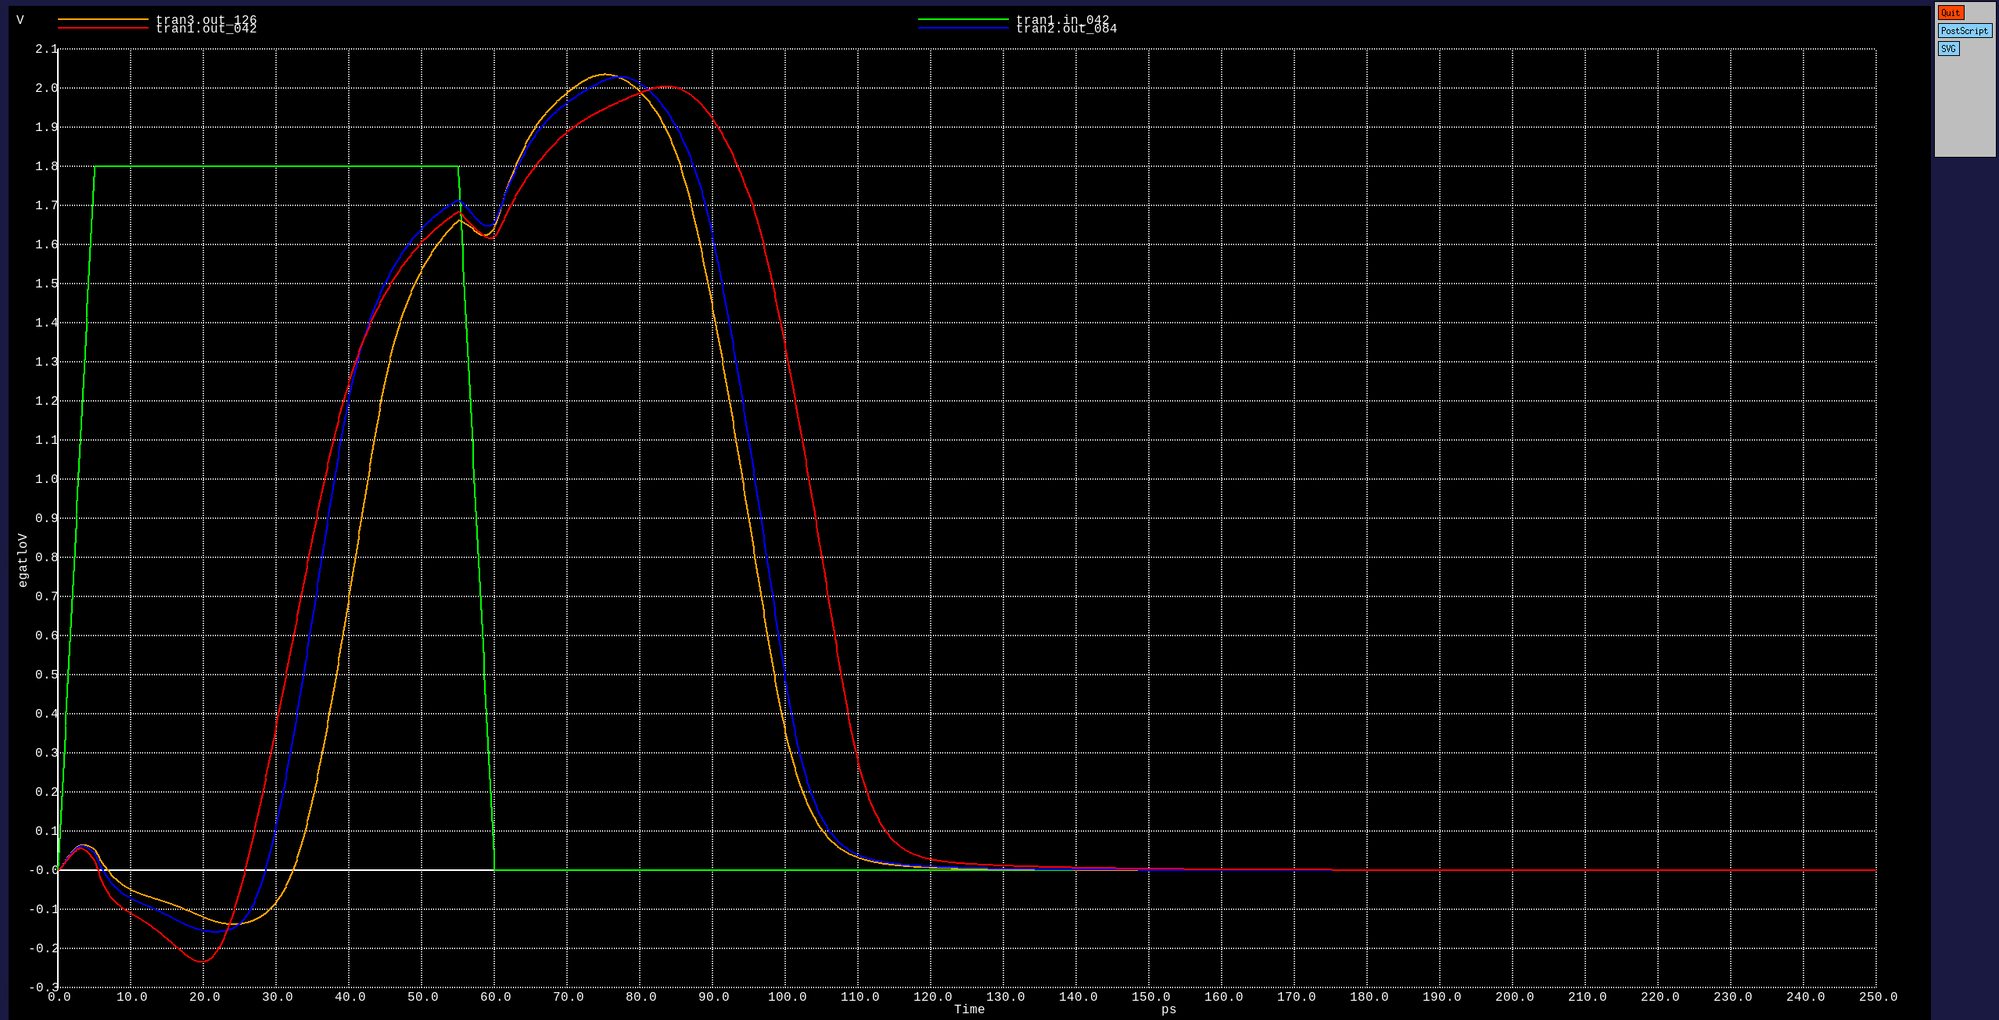
\includegraphics[width=0.9\textwidth]{figures/1a_tran.png}
  \caption{Simulated $V_{out}$ transient response to the input PULSE (green:
  \texttt{v(inp)}), overlaid for the three swept $W_p$ values -- blue
  $W_p=0.84\ \mu\text{m}$, red $W_p=1.26\ \mu\text{m}$, orange (underneath)
  $W_p=0.42\ \mu\text{m}$. The output has no further fan-out, so it swings
  well above $V_{DD}=1.8$~V transiently (overshoot to $\approx2.0$--$2.1$~V)
  before settling back.}
  \label{fig:1a-tran}
\end{figure}

\begin{table}[h]
  \centering
  \begin{tabular}{|c|c|c|c|}
    \hline
    $W_p$ ($\mu$m) & $t_{LH}$ (ps) & $t_{HL}$ (ps) & Simulated $t_p$ (ps) \\
    \hline
    0.42 & 33.02 & 46.62 & 39.82 \\
    \textbf{0.84} & 34.61 & 39.13 & \textbf{36.87} \\
    1.26 & 39.21 & 37.46 & 38.34 \\
    \hline
  \end{tabular}
  \caption{Simulated delay vs.\ $W_p$, from the
  \texttt{delay\_042}/\texttt{084}/\texttt{126} \texttt{meas} statements in
  \texttt{assign1a.spice} (ngspice log, minimum in bold). Note
  \texttt{tlh\_XXX}/\texttt{thl\_XXX} here are \emph{trig(v(inp))}$\to$
  \emph{targ(v(out))} same-polarity-edge measurements -- since \texttt{out} is
  two inversions downstream of \texttt{inp} (\texttt{x1}: \texttt{inp}
  $\to$\texttt{net1}, \texttt{x2}: \texttt{net1}$\to$\texttt{out}), each is
  really the sum of one stage's $t_{pHL}$ and the other's $t_{pLH}$, not a
  single-stage delay.}
  \label{tab:1a-sim}
\end{table}

\paragraph{Discussion.} The simulated delay is \textbf{non-monotonic} in
$W_p$, with a clear minimum at $W_p=0.84\ \mu\text{m}$ ($36.87$~ps) --
confirming the hypothesis above and the \texttt{width\_p=0.84} default carried
into Parts 1(b)/(c) and Problem 2 -- rather than falling monotonically as the
fixed-$C_{tot}$ analytical model (Table~\ref{tab:1a-analytical}) predicts. The
simulated values are also uniformly $\sim2$--$4\times$ larger than that
analytical estimate ($36.9$--$39.8$~ps simulated vs.\ $10.0$--$19.6$~ps
analytical), consistent with the same order of long-channel/velocity-
saturation model error seen throughout Assignments 1--2.

Two effects the fixed-$C_{tot}$, single-stage model omits explain the
non-monotonicity: (1) as noted in Table~\ref{tab:1a-sim}, each measured
\texttt{tlh}/\texttt{thl} is actually a \emph{two-stage} delay
($t_{pHL,\text{stage1}}+t_{pLH,\text{stage2}}$ or vice versa), so it mixes a
Wp-independent nMOS delay with a Wp-\emph{dependent} pMOS delay \emph{and} a
Wp-dependent load, since stage 1 drives stage 2's gate capacitance, which
itself scales with $W_p$ (both stages share the same \texttt{width\_p}); and
(2) consequently, growing $W_p$ from $0.84$ to $1.26\ \mu\text{m}$ still
strengthens each stage's own pull-up, but now also enlarges every
inter-stage gate load enough that the net delay ticks back up rather than
continuing to fall -- exactly the self/fan-out loading trade-off flagged
above. $W_p=0.84\ \mu\text{m}$ (i.e.\ $(W/L)_p=5.6$, $2\times(W/L)_n$) is
therefore carried forward as the minimum-delay sizing for the rest of this
report.

\subsection{Part (b): Propagation Delay vs.\ $V_{DD}$ ($1.0$--$1.8$~V)}

Using the minimum-delay $W_p$ from Part (a) ($W_p=0.84\ \mu\text{m}$, confirmed
above and matching the value hard-coded in \texttt{assign1b.spice}), plot
$t_p$ vs.\ $V_{DD}$ for $V_{DD}=1.0$ to $1.8$~V in $0.1$~V steps, and
compare against the analytical estimate.

\subsubsection{Calculation}

With $(W/L)_p=5.6$ fixed, $K_p'(W/L)_p = 411.3\ \mu\text{A/V}^2$. Applying the
averaged-current model of Section~1 (with the script's constants
$L_n\xi_{c,n}=0.96$~V, $L_p\xi_{c,p}=1.0$~V) across the swept $V_{DD}$ gives
Table~\ref{tab:1b-analytical}.

\begin{table}[h]
  \centering
  \begin{tabular}{|c|c|c|c|}
    \hline
    $V_{DD}$ (V) & $t_{pHL}$ (ps) & $t_{pLH}$ (ps) & $t_p$ (ps) \\
    \hline
    1.0 & 47.46 & 66.74 & 57.10 \\
    1.1 & 31.70 & 44.47 & 38.09 \\
    1.2 & 23.76 & 33.27 & 28.51 \\
    1.3 & 19.10 & 26.70 & 22.90 \\
    1.4 & 16.08 & 22.44 & 19.26 \\
    1.5 & 13.98 & 19.49 & 16.74 \\
    1.6 & 12.46 & 17.34 & 14.90 \\
    1.7 & 11.30 & 15.71 & 13.50 \\
    1.8 & 10.39 & 14.44 & 12.41 \\
    \hline
  \end{tabular}
  \caption{Analytical $t_p$ vs.\ $V_{DD}$, $W_p=0.84\ \mu\text{m}$
  (averaged-current model, script constants).}
  \label{tab:1b-analytical}
\end{table}

As $V_{DD}$ falls, the $(V_{DD}-V_T)^2$ term in the denominator of $I_{av}$
shrinks much faster than the $V_{DD}/2$ numerator shrinks, so $t_p$ grows
sharply toward low $V_{DD}$ -- roughly $4.6\times$ from $1.8$~V down to
$1.0$~V in this idealized model.

\subsubsection{Schematic}

The topology reuses \texttt{inverter.sch} for the load stage and
\texttt{ignd.sch} (\texttt{inverter.sch} plus a grounded-through-ammeter
\texttt{to\_gnd} tap, sensed via a $0$~V \texttt{Vmeas} source) for the driving
stage, so that the supply current needed for Part 1(c)'s energy calculation is
available from the same sweep.

\begin{figure}[h]
  \centering
  
\includegraphics[width=0.9\textwidth]{figures/1b_schematic.png}
  \caption{FO1 inverter pair with the driving stage's supply current sensed
  via \texttt{ignd} + \texttt{Vmeas}, and \texttt{VDD} parametrized for the
  sweep.}
  \label{fig:1b-schematic}
\end{figure}

\subsubsection{Measurement}

\texttt{assign1b.spice} sweeps $V_{DD}$ (via \texttt{alterparam} + \texttt{reset})
and extracts both the simulated delay and the in-line analytical estimate at
each point. Unlike Part (a)'s \texttt{v(out)} target (two inversions
downstream of \texttt{v(inp)}), here \texttt{meas} targets \texttt{v(net1)}
directly -- the \texttt{ignd} driving stage's own output -- so
\texttt{thl}/\texttt{tlh} are genuine single-stage $t_{pHL}$/$t_{pLH}$,
directly comparable to the Calculation model above:

\begin{verbatim}
.control
let Nsim = 9
let delayvec = vector(Nsim)
let delayvec_ana = vector(Nsim)
let vddvec = vector(Nsim)
let index = 0

let Ctot = 3.8e-15
let Vtn = 0.7
let Vtp = 0.7
let EcnLn = 0.96
let EcpLp = 1.0
let Kn_WL = 5.838e-4
let Kp_WL = 4.112e-4

while index < Nsim
  let vddv = 1.0 + (index * 0.1)
  let vby2 = vddv / 2
  alterparam VDDVal = $&vddv
  reset
  tran 1p 600p

  meas tran thl trig v(inp) val=$&vby2 rise=1 targ v(net1) val=$&vby2 fall=1
  meas tran tlh trig v(inp) val=$&vby2 fall=1 targ v(net1) val=$&vby2 rise=1
  let delayvec[index] = (thl + tlh) / 2

  let num_hl = Ctot * vby2 * (EcnLn + vddv - Vtn)
  let den_hl = Kn_WL * EcnLn * (vddv - Vtn) * (vddv - Vtn)
  let tphl_ana = num_hl / den_hl
  let num_lh = Ctot * vby2 * (EcpLp + vddv - Vtp)
  let den_lh = Kp_WL * EcpLp * (vddv - Vtp) * (vddv - Vtp)
  let tplh_ana = num_lh / den_lh
  let delayvec_ana[index] = (tphl_ana + tplh_ana) / 2

  let vddvec[index] = vddv
  let index = index + 1
end

plot delayvec delayvec_ana vs vddvec
.endc
\end{verbatim}

\begin{figure}[h]
  \centering
  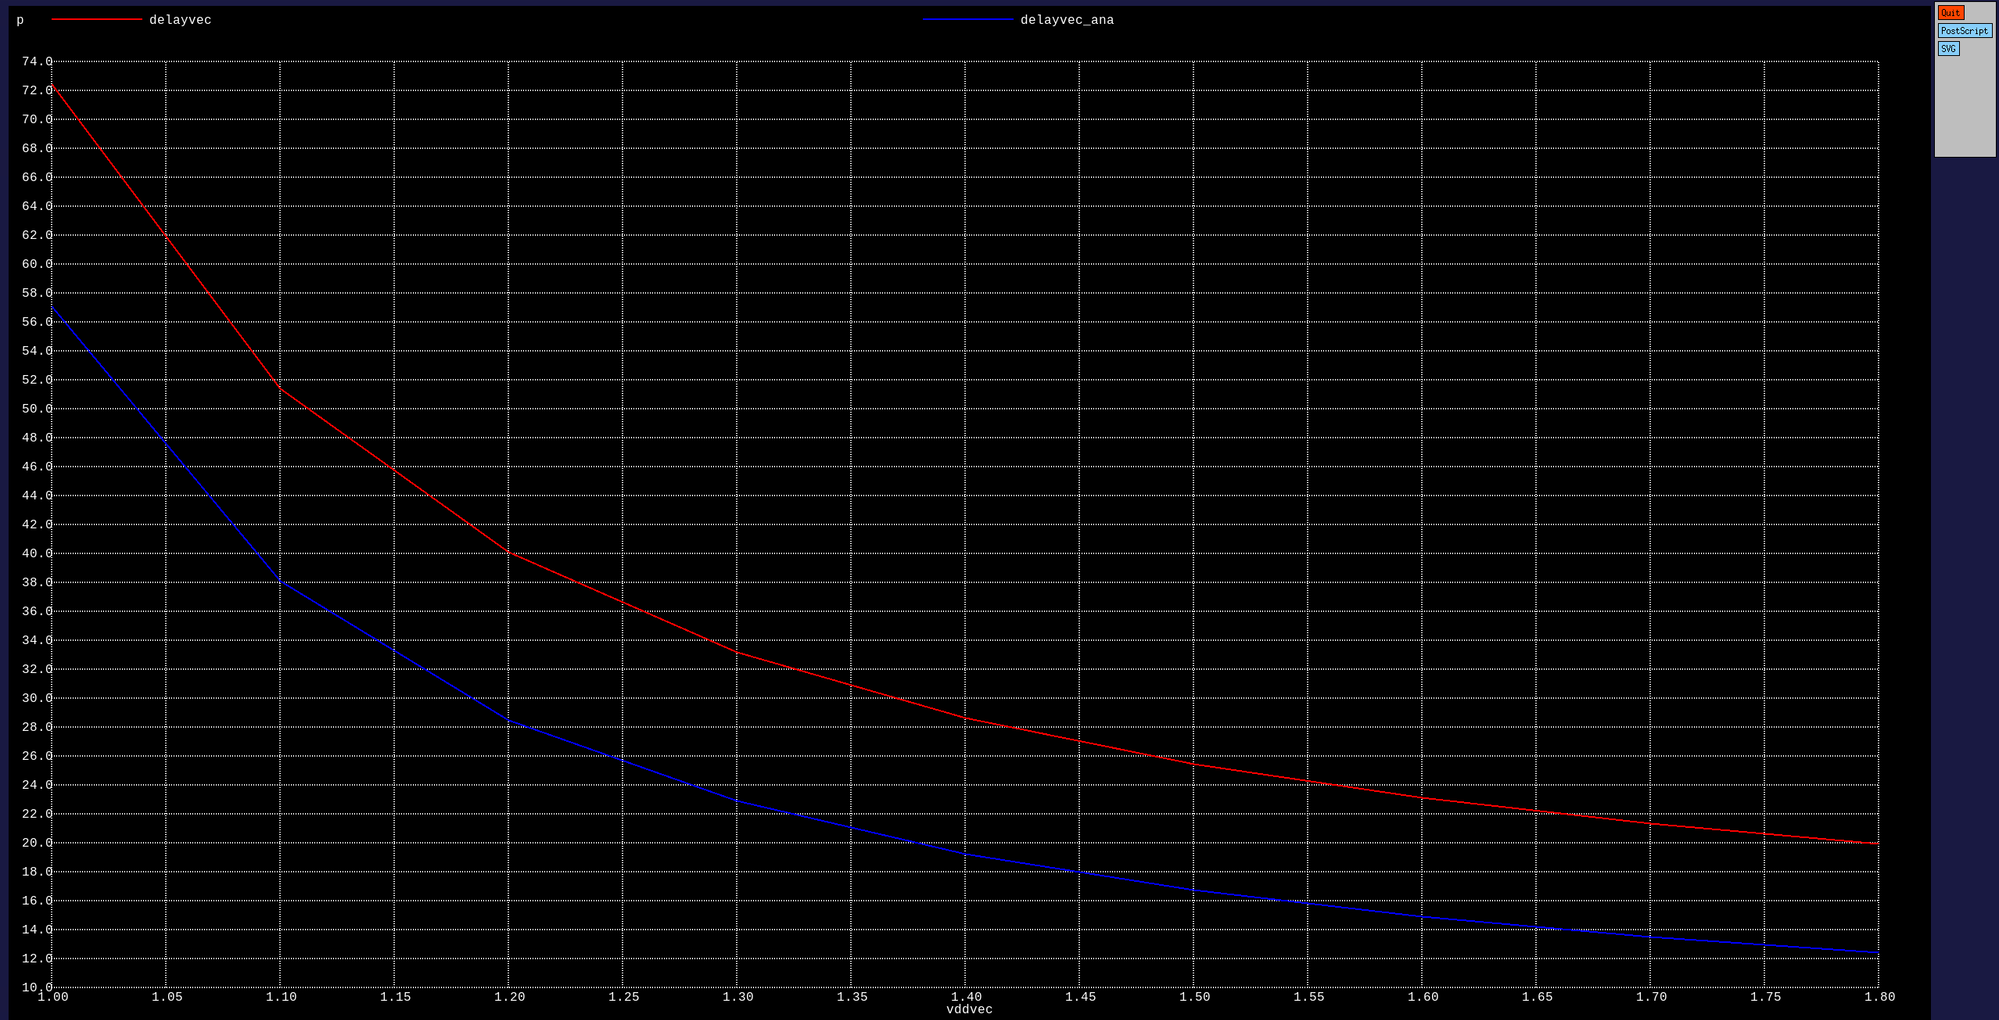
\includegraphics[width=0.9\textwidth]{figures/1b_delay.png}
  \caption{Simulated (\texttt{delayvec}, red) vs.\ in-line analytical
  (\texttt{delayvec\_ana}, blue) $t_p$ vs.\ $V_{DD}$.}
  \label{fig:1b-plot}
\end{figure}

\begin{table}[h]
  \centering
  \begin{tabular}{|c|c|c|c|}
    \hline
    $V_{DD}$ (V) & Simulated $t_p$ (ps) & Analytical $t_p$ (ps) & Ratio (sim/ana) \\
    \hline
    1.0 & $\approx72$\textsuperscript{*} & 57.10 & 1.26 \\
    1.1 & $\approx52$\textsuperscript{*} & 38.09 & 1.37 \\
    1.2 & $\approx40$\textsuperscript{*} & 28.51 & 1.40 \\
    1.3 & 33.21 & 22.90 & 1.45 \\
    1.4 & 28.66 & 19.26 & 1.49 \\
    1.5 & 25.46 & 16.74 & 1.52 \\
    1.6 & 23.11 & 14.90 & 1.55 \\
    1.7 & 21.33 & 13.50 & 1.58 \\
    1.8 & 19.94 & 12.41 & 1.61 \\
    \hline
  \end{tabular}
  \caption{Simulated (\texttt{delayvec}) vs.\ analytical (\texttt{delayvec\_ana})
  $t_p$ vs.\ $V_{DD}$. Rows marked \textsuperscript{*} ($V_{DD}=1.0$--$1.2$~V)
  are read off Figure~\ref{fig:1b-plot} (the ngspice log for these three
  iterations scrolled out of the captured terminal buffer); $V_{DD}=1.3$--$1.8$~V
  are exact values from the \texttt{meas} log.}
  \label{tab:1b-sim}
\end{table}

\paragraph{Discussion.} The simulated and analytical curves
(Figure~\ref{fig:1b-plot}, Table~\ref{tab:1b-sim}) track each other closely in
shape -- both rise sharply toward low $V_{DD}$ and nearly overlap for
$V_{DD}\lesssim1.15$~V -- but the analytical curve is a systematic
\emph{underestimate} that gets proportionally worse at higher $V_{DD}$: the
sim/analytical ratio grows monotonically from $1.26\times$ at $V_{DD}=1.0$~V
to $1.61\times$ at $V_{DD}=1.8$~V. This is the opposite trend from a constant
percentage-error model error -- it suggests the averaged-current
approximation (evaluating $I_{av}$ at a single fixed overdrive $V_{gt}=V_{DD}-V_T$
rather than integrating the actual time-varying current through the
transition) increasingly underestimates the true switching charge/delay as
the full swing $V_{DD}$ grows relative to $V_T$, consistent with the same
kind of averaged/peak-current approximation gap discussed for the
$I_{DS}$ estimate in Assignment 2, Part 1(d).

\subsection{Part (c): Energy-Delay Product vs.\ $V_{DD}$}

\subsubsection{Calculation}

Energy per transition is approximated as $E\approx C_{tot}V_{DD}^2$ (full
rail-to-rail switching energy), so $EDP = C_{tot}V_{DD}^2\,t_p(V_{DD})$ using
the $t_p(V_{DD})$ of Table~\ref{tab:1b-analytical}.

\begin{table}[h]
  \centering
  \begin{tabular}{|c|c|c|}
    \hline
    $V_{DD}$ (V) & $t_p$ (ps) & $EDP$ (fJ$\cdot$ps) \\
    \hline
    1.0 & 57.10 & 216.99 \\
    1.1 & 38.09 & 175.12 \\
    1.2 & 28.51 & 156.02 \\
    1.3 & 22.90 & 147.05 \\
    1.4 & 19.26 & \textbf{143.46} \\
    1.5 & 16.74 & \textbf{143.12} \\
    1.6 & 14.90 & 144.93 \\
    1.7 & 13.50 & 148.29 \\
    1.8 & 12.41 & 152.81 \\
    \hline
  \end{tabular}
  \caption{Analytical $EDP=C_{tot}V_{DD}^2\,t_p$ vs.\ $V_{DD}$
  ($C_{tot}=3.8$~fF). Minimum in bold.}
  \label{tab:1c-analytical}
\end{table}

The analytical $EDP$ is a shallow, roughly U-shaped curve with a minimum near
$V_{DD}\approx1.4$--$1.5$~V ($\approx143$~fJ$\cdot$ps) -- i.e.\ the model
predicts the energy-delay-optimal supply voltage sits noticeably \emph{below}
the nominal $1.8$~V rail: below $\approx1.4$~V, $t_p$ grows faster than
$V_{DD}^2$ falls (energy savings are outweighed by the delay penalty);
above $\approx1.5$~V, $t_p$ is nearly flat while $V_{DD}^2$ keeps growing, so
$EDP$ rises again.

\subsubsection{Schematic}

Identical topology to Part (b) (Figure~\ref{fig:1b-schematic}): the
\texttt{ignd} driving stage's supply current is sensed via \texttt{Vmeas} and
integrated over the transient to get the switching charge.

\begin{figure}[h]
  \centering
  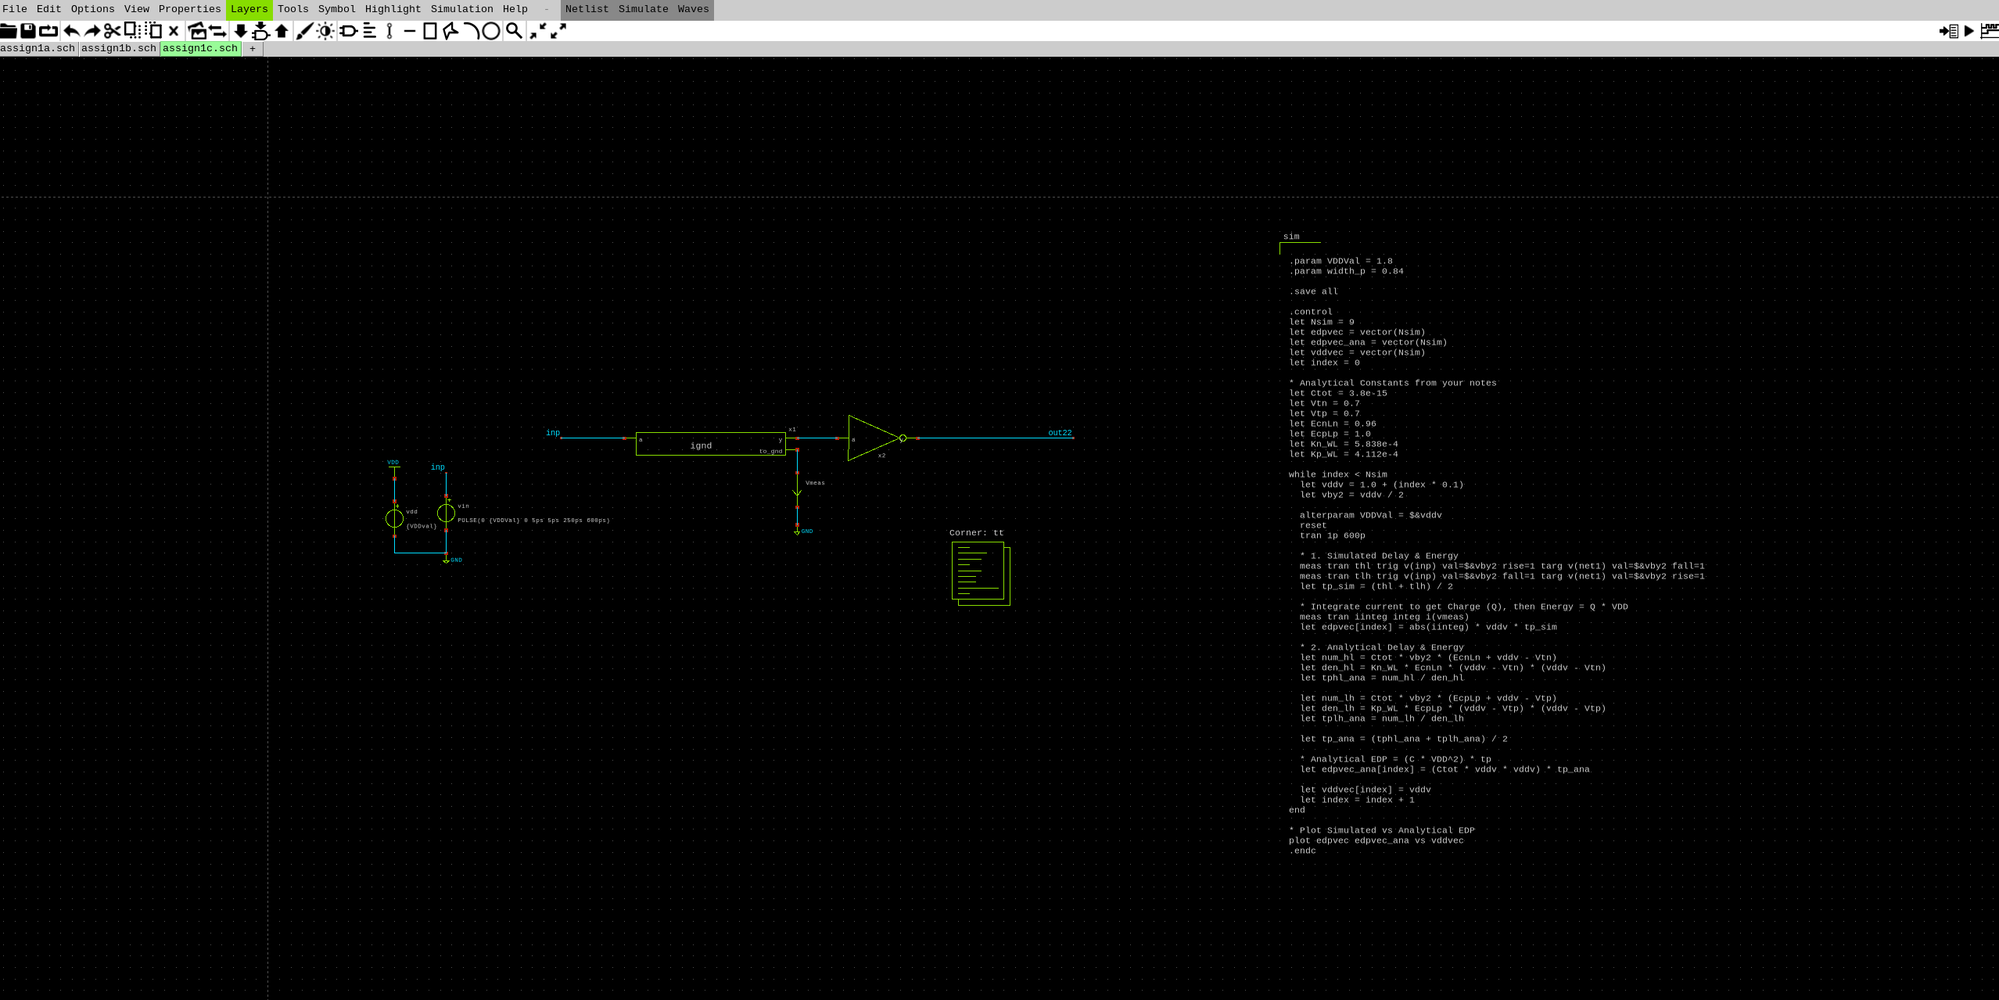
\includegraphics[width=0.9\textwidth]{figures/1c_schematic.png}
  \caption{\texttt{assign1c.sch} -- same FO1 pair and current-sense tap as
  Part (b), \texttt{VDD} parametrized for the sweep.}
  \label{fig:1c-schematic}
\end{figure}

\subsubsection{Measurement}

\texttt{assign1c.spice} extends the same sweep with a charge integration
(\texttt{meas tran iinteg integ i(vmeas)}) to get simulated energy directly:

\begin{verbatim}
* (same VDD sweep/reset/tran structure as assign1b.spice)
meas tran iinteg integ i(vmeas)
let edpvec[index] = abs(iinteg) * vddv * tp_sim

let edpvec_ana[index] = (Ctot * vddv * vddv) * tp_ana

plot edpvec edpvec_ana vs vddvec
.endc
\end{verbatim}

\begin{figure}[h]
  \centering
  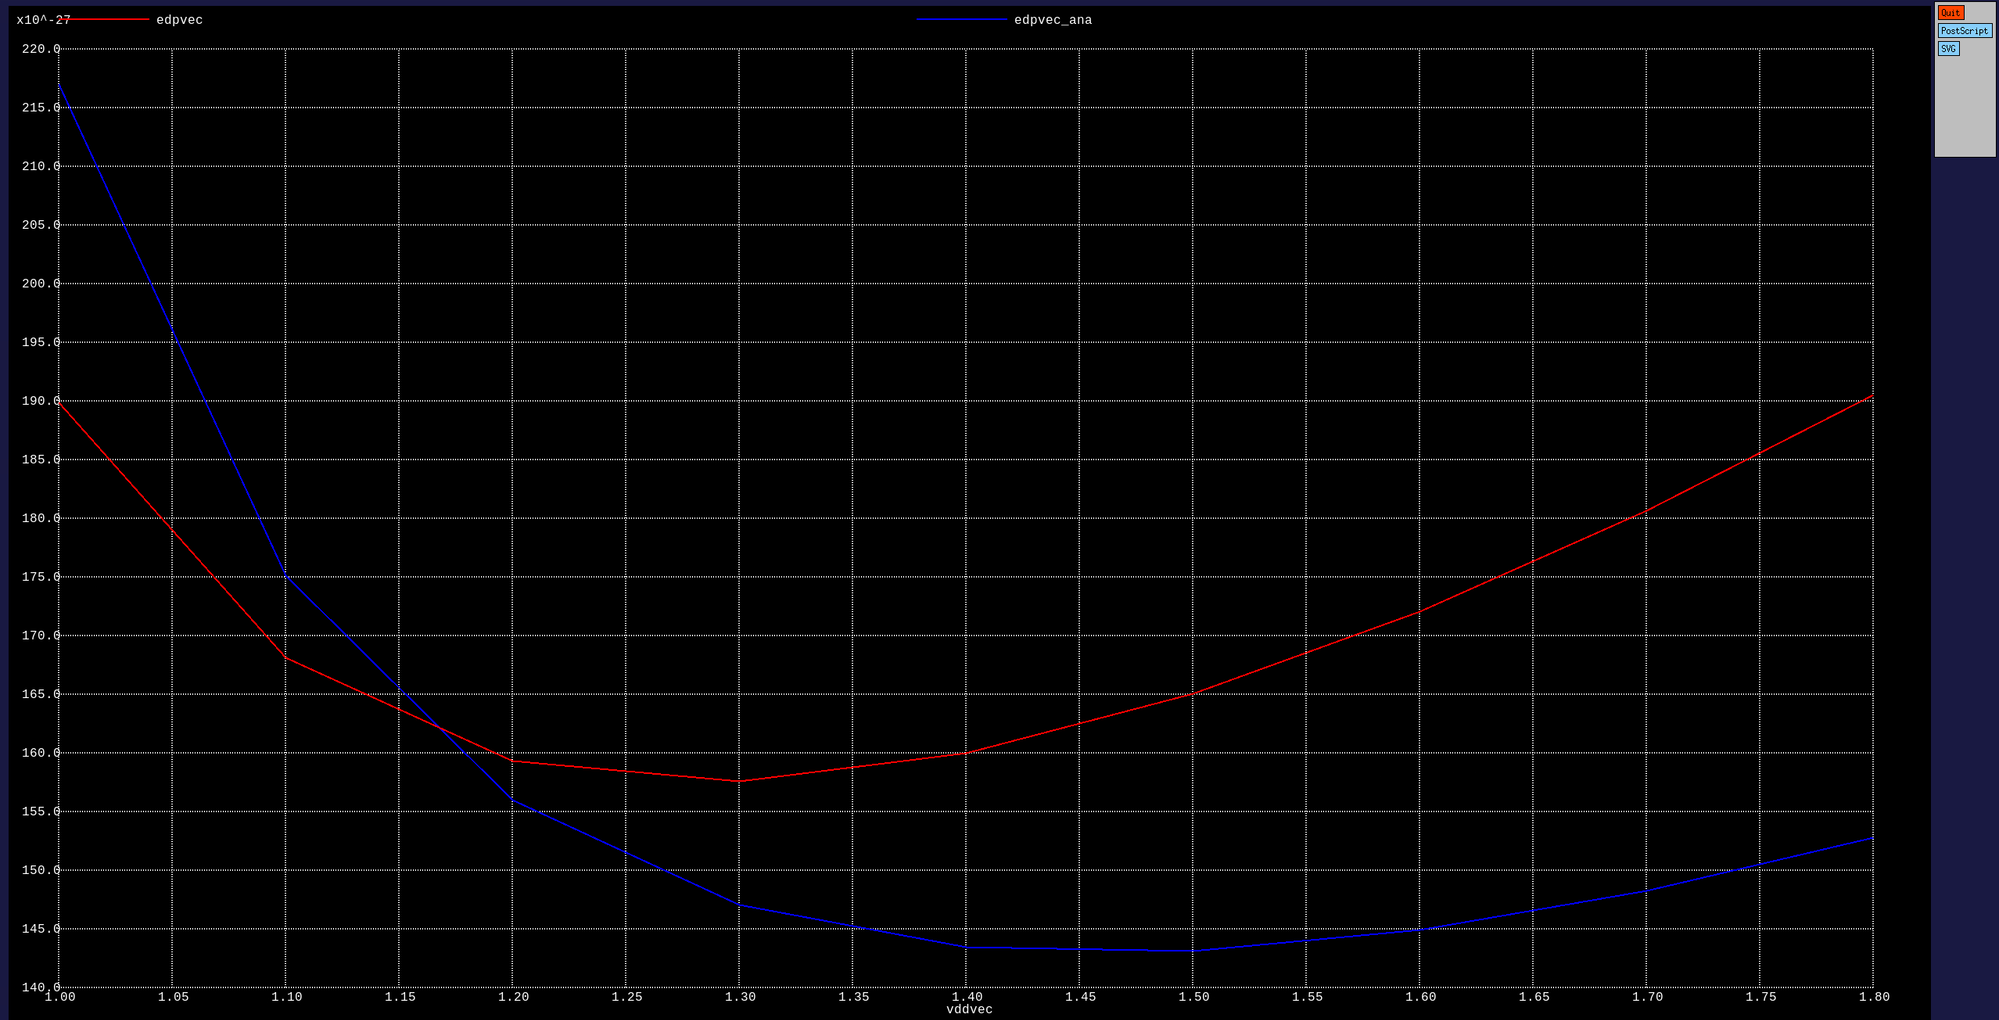
\includegraphics[width=0.9\textwidth]{figures/1c_edp.png}
  \caption{Simulated (\texttt{edpvec}, red) vs.\ analytical
  (\texttt{edpvec\_ana}, blue) energy-delay product vs.\ $V_{DD}$.}
  \label{fig:1c-plot}
\end{figure}

\begin{table}[h]
  \centering
  \begin{tabular}{|c|c|c|c|}
    \hline
    $V_{DD}$ (V) & Simulated $EDP$ (fJ$\cdot$ps) & Analytical $EDP$ (fJ$\cdot$ps) & $Q_{sim}$ (fC) \\
    \hline
    1.0 & $\approx190$\textsuperscript{*} & 216.99 & -- \\
    1.1 & $\approx175$\textsuperscript{*} & 175.12 & -- \\
    1.2 & $\approx160$\textsuperscript{*} & 156.02 & -- \\
    1.3 & \textbf{157.63} & 147.05 & 3.651 \\
    1.4 & 160.00 & \textbf{143.46} & 3.988 \\
    1.5 & 165.04 & \textbf{143.12} & 4.322 \\
    1.6 & 172.05 & 144.93 & 4.653 \\
    1.7 & 180.66 & 148.29 & 4.982 \\
    1.8 & 190.55 & 152.81 & 5.309 \\
    \hline
  \end{tabular}
  \caption{Simulated (\texttt{edpvec}) vs.\ analytical (\texttt{edpvec\_ana})
  $EDP$ vs.\ $V_{DD}$; $Q_{sim}=$\texttt{iinteg} is the driving stage's
  integrated supply charge over the $600$~ps transient window. Rows marked
  \textsuperscript{*} ($V_{DD}=1.0$--$1.2$~V) are read off
  Figure~\ref{fig:1c-plot} (same scrolled-off log as Part (b));
  $V_{DD}=1.3$--$1.8$~V are exact \texttt{meas}/\texttt{let} values.
  Per-curve minimum in bold.}
  \label{tab:1c-sim}
\end{table}

\paragraph{Discussion.} The simulated $EDP$ minimum sits at
$V_{DD}\approx1.3$~V ($157.6$~fJ$\cdot$ps, and nearly flat out to $1.4$~V at
$160.0$~fJ$\cdot$ps) -- \emph{lower} than the analytical optimum of
$V_{DD}\approx1.4$--$1.5$~V ($\approx143$~fJ$\cdot$ps). The two curves cross
near $V_{DD}\approx1.15$~V (Figure~\ref{fig:1c-plot}): for $V_{DD}\lesssim1.15$~V
the simulated $EDP$ is actually \emph{below} the analytical curve, but for
$V_{DD}\gtrsim1.15$~V it sits increasingly \emph{above} it, reaching $190.6$
vs.\ $152.8$~fJ$\cdot$ps ($\approx25\%$ higher) at the nominal $V_{DD}=1.8$~V.
This is a direct consequence of Part (b)'s finding: simulated $t_p$ is an
increasingly larger multiple of the analytical $t_p$ as $V_{DD}$ rises
(Table~\ref{tab:1b-sim}), and since $EDP\propto t_p$ at fixed charge, that
same growing gap propagates directly into $EDP$ and pulls its minimum to a
lower $V_{DD}$ than the (systematically delay-underestimating) analytical
model predicts. Practically, this means the analytical velocity-saturation
model is directionally right about there being an energy-delay-optimal
$V_{DD}$ well below the $1.8$~V rail, but modestly overstates \emph{how high}
that optimum sits ($\approx1.4$--$1.5$~V analytically vs.\ $\approx1.3$~V
simulated) -- and, more importantly, understates the $EDP$ penalty of running
at the full $1.8$~V rail instead ($152.8$~fJ$\cdot$ps analytical vs.\
$190.6$~fJ$\cdot$ps simulated, i.e.\ the real relative benefit of moving off
$V_{DD}=1.8$~V toward the optimum is understated by the same
$\approx25\%$).

\section{Problem 2: Ring Oscillator}

Using the minimum-delay inverter from Problem 1(a) ($W_p=0.84\ \mu\text{m}$),
a ring of $N$ identical inverters is closed on itself
(\texttt{assign2a.sch}: \texttt{x1}--\texttt{x7}, each stage's output driving
the next, the last driving the first). Oscillation is seeded with
\texttt{.ic v(vout)=0} so the odd-inverter-count ring does not sit at a
(metastable) fixed point.

\paragraph{Analytical frequency.} For an $N$-stage ring oscillator, the loop
must accumulate a total delay of one half-period per full logic inversion
around the loop, giving the standard estimate
\[
f_{osc} = \frac{1}{2\,N\,t_p},
\]
using the same per-stage $t_p(V_{DD})$ from Problem 1(b) (Table~\ref{tab:1b-analytical}).

\subsection{Part (a): Oscillation Frequency at $V_{DD}=1.8$~V, $N=7$}

\subsubsection{Calculation}

Using $t_p(1.8\text{V})=12.41$~ps from Table~\ref{tab:1b-analytical} and $N=7$:
\[
f_{osc} = \frac{1}{2\times7\times12.41\text{ps}} \approx 5.75\ \text{GHz},
\qquad T = 1/f_{osc} \approx 173.8\ \text{ps}.
\]

\subsubsection{Schematic}

\begin{figure}[h]
  \centering
  
\includegraphics[width=0.95\textwidth]{figures/2a_schematic.png}
  \caption{7-stage ring oscillator (\texttt{assign2a.sch}, \texttt{x1}--\texttt{x7})
  built from the Problem 1 inverter ($W_p=0.84\ \mu\text{m}$), closed on
  itself into \texttt{vout}.}
  \label{fig:2a-schematic}
\end{figure}

\subsubsection{Measurement}

\begin{verbatim}
.ic v(vout)=0

.control
tran 1p 5n uic
meas tran t1 WHEN v(vout)=0.9 rise=4
meas tran t2 WHEN v(vout)=0.9 rise=5
let period = t2 - t1
let freq = 1 / period
print period
print freq
plot v(vout)
.endc
\end{verbatim}

\begin{figure}[h]
  \centering
  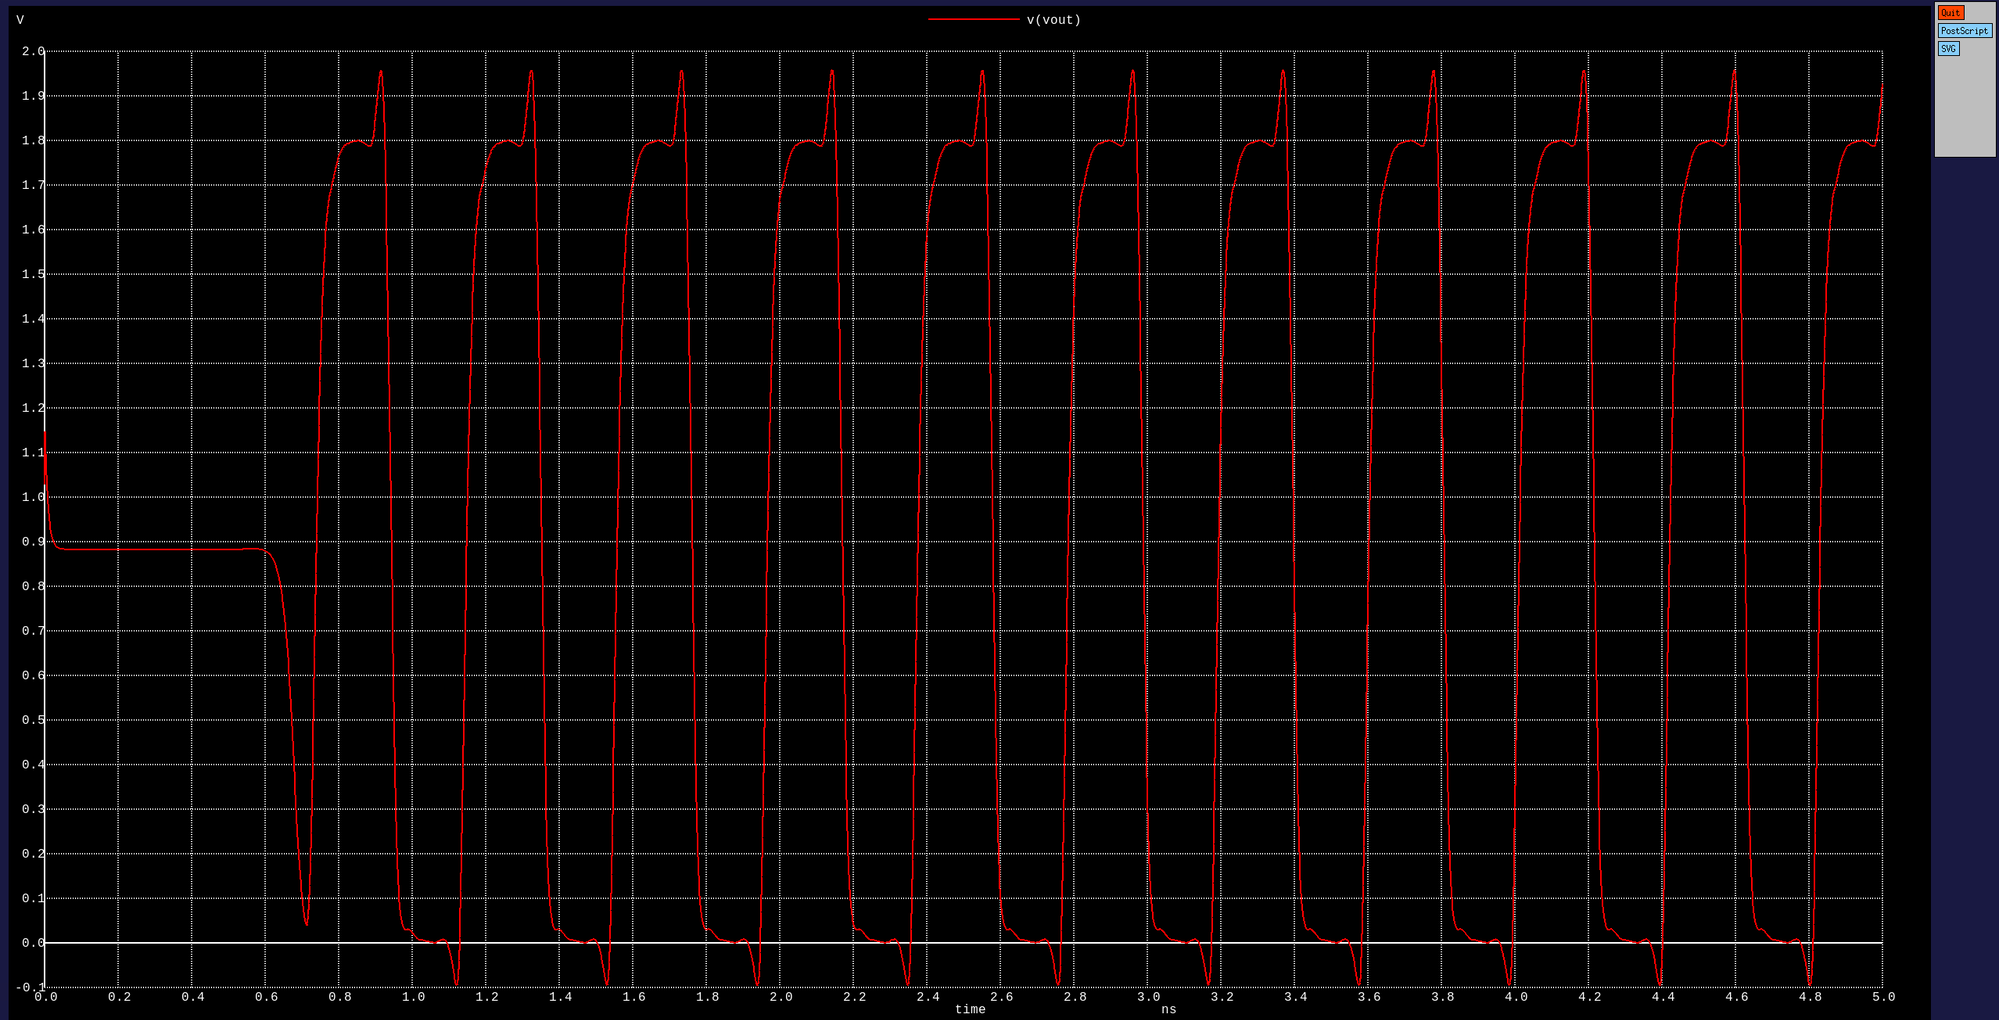
\includegraphics[width=0.95\textwidth]{figures/2a_waveform.png}
  \caption{Simulated ring-oscillator output $v(vout)$ at $V_{DD}=1.8$~V. Note
  the transient overshoot/undershoot beyond the $0$--$1.8$~V rails on every
  cycle -- the node never fully settles before the next transition begins.}
  \label{fig:2a-waveform}
\end{figure}

\begin{table}[h]
  \centering
  \begin{tabular}{|l|c|c|}
    \hline
    Quantity & Analytical & Simulated \\
    \hline
    Period $T$ & 173.8 ps & 409.12 ps \\
    Frequency $f_{osc}$ & 5.75 GHz & 2.444 GHz \\
    \hline
  \end{tabular}
  \caption{Analytical vs.\ simulated 7-stage ring oscillator period/frequency
  at $V_{DD}=1.8$~V. Simulated values from the \texttt{period}/\texttt{freq}
  \texttt{print} output ($t_1=1.9663$~ns, $t_2=2.3754$~ns, 4th/5th rising
  edges of $v(vout)=0.9$~V -- chosen well after the first cycle so the ring
  has settled into steady-state oscillation).}
  \label{tab:2a-sim}
\end{table}

\paragraph{Discussion.} The simulated oscillation is $2.35\times$ slower than
the analytical estimate ($2.444$~GHz vs.\ $5.75$~GHz simulated/analytical, or
equivalently $T=409.1$~ps vs.\ $173.8$~ps). Backing out an effective
per-stage delay from the simulated period, $t_{p,\text{eff}} = T/(2N) =
409.1/14 = 29.2$~ps -- itself $1.47\times$ \emph{larger} than the single-stage
FO1 delay directly measured in Part 1(b) at the same $V_{DD}$ ($19.94$~ps,
Table~\ref{tab:1b-sim}), even though both circuits use the identical inverter
sizing and (effectively) the same FO1 loading. The extra gap beyond Part
1(b)'s already-larger-than-analytical delay is consistent with
Figure~\ref{fig:2a-waveform}: unlike Part 1(b)'s single clean pulse response
settling to a quiescent rail, the ring's node never fully settles between
transitions (visible rail-overshoot/undershoot every cycle, and the high
phase sits at a shallower, rounded plateau rather than a flat $1.8$~V) --
i.e.\ each stage is repeatedly re-triggered from a partially-settled state
rather than from a clean $0$/$V_{DD}$ starting point, which is exactly the
kind of steady-state loading effect a single-transition delay measurement
(Part 1(b)) or a static per-stage formula (this section's Calculation) cannot
capture.

\subsection{Part (b): Frequency/Period vs.\ $V_{DD}$, $N=7$}

\subsubsection{Calculation}

Applying $f_{osc}=1/(2\,N\,t_p(V_{DD}))$ with $N=7$ to
Table~\ref{tab:1b-analytical}:

\begin{table}[h]
  \centering
  \begin{tabular}{|c|c|c|c|}
    \hline
    $V_{DD}$ (V) & $t_p$ (ps) & $f_{osc}$ (GHz) & $T$ (ps) \\
    \hline
    1.0 & 57.10 & 1.251 & 799.4 \\
    1.1 & 38.09 & 1.875 & 533.2 \\
    1.2 & 28.51 & 2.505 & 399.2 \\
    1.3 & 22.90 & 3.120 & 320.6 \\
    1.4 & 19.26 & 3.708 & 269.7 \\
    1.5 & 16.74 & 4.267 & 234.3 \\
    1.6 & 14.90 & 4.794 & 208.6 \\
    1.7 & 13.50 & 5.290 & 189.0 \\
    1.8 & 12.41 & 5.755 & 173.8 \\
    \hline
  \end{tabular}
  \caption{Analytical 7-stage ring oscillator frequency/period vs.\ $V_{DD}$.}
  \label{tab:2b-analytical}
\end{table}

\subsubsection{Schematic}

\begin{figure}[h]
  \centering
  
\includegraphics[width=0.95\textwidth]{figures/2b_schematic.png}
  \caption{7-stage ring oscillator (\texttt{assign2b.sch}), identical to
  Figure~\ref{fig:2a-schematic} but with \texttt{VDD} parametrized
  (\texttt{vdd\_val}) for the sweep.}
  \label{fig:2b-schematic}
\end{figure}

\subsubsection{Measurement}

\texttt{assign2b.spice} sweeps \texttt{vdd\_val} the same way as
\texttt{assign1b.spice}, but measures 5 rising edges of the (now periodic)
\texttt{v(vout)} to extract period/frequency directly:

\begin{verbatim}
.control
let Nsim = 9
let periodvec = vector(Nsim)
let freqvec = vector(Nsim)
let vddvec = vector(Nsim)
let index = 0

while index < Nsim
  let vddv = 1.0 + (index * 0.1)
  alterparam vdd_val = $&vddv
  reset
  tran 1p 100n uic
  meas tran t1 WHEN v(vout)=0.4 rise=4
  meas tran t2 WHEN v(vout)=0.4 rise=5
  let periodvec[index] = t2 - t1
  let freqvec[index] = 1 / (t2 - t1)
  let vddvec[index] = vddv
  let index = index + 1
end

plot freqvec vs vddvec
plot periodvec vs vddvec
.endc
\end{verbatim}

\begin{figure}[h]
  \centering
  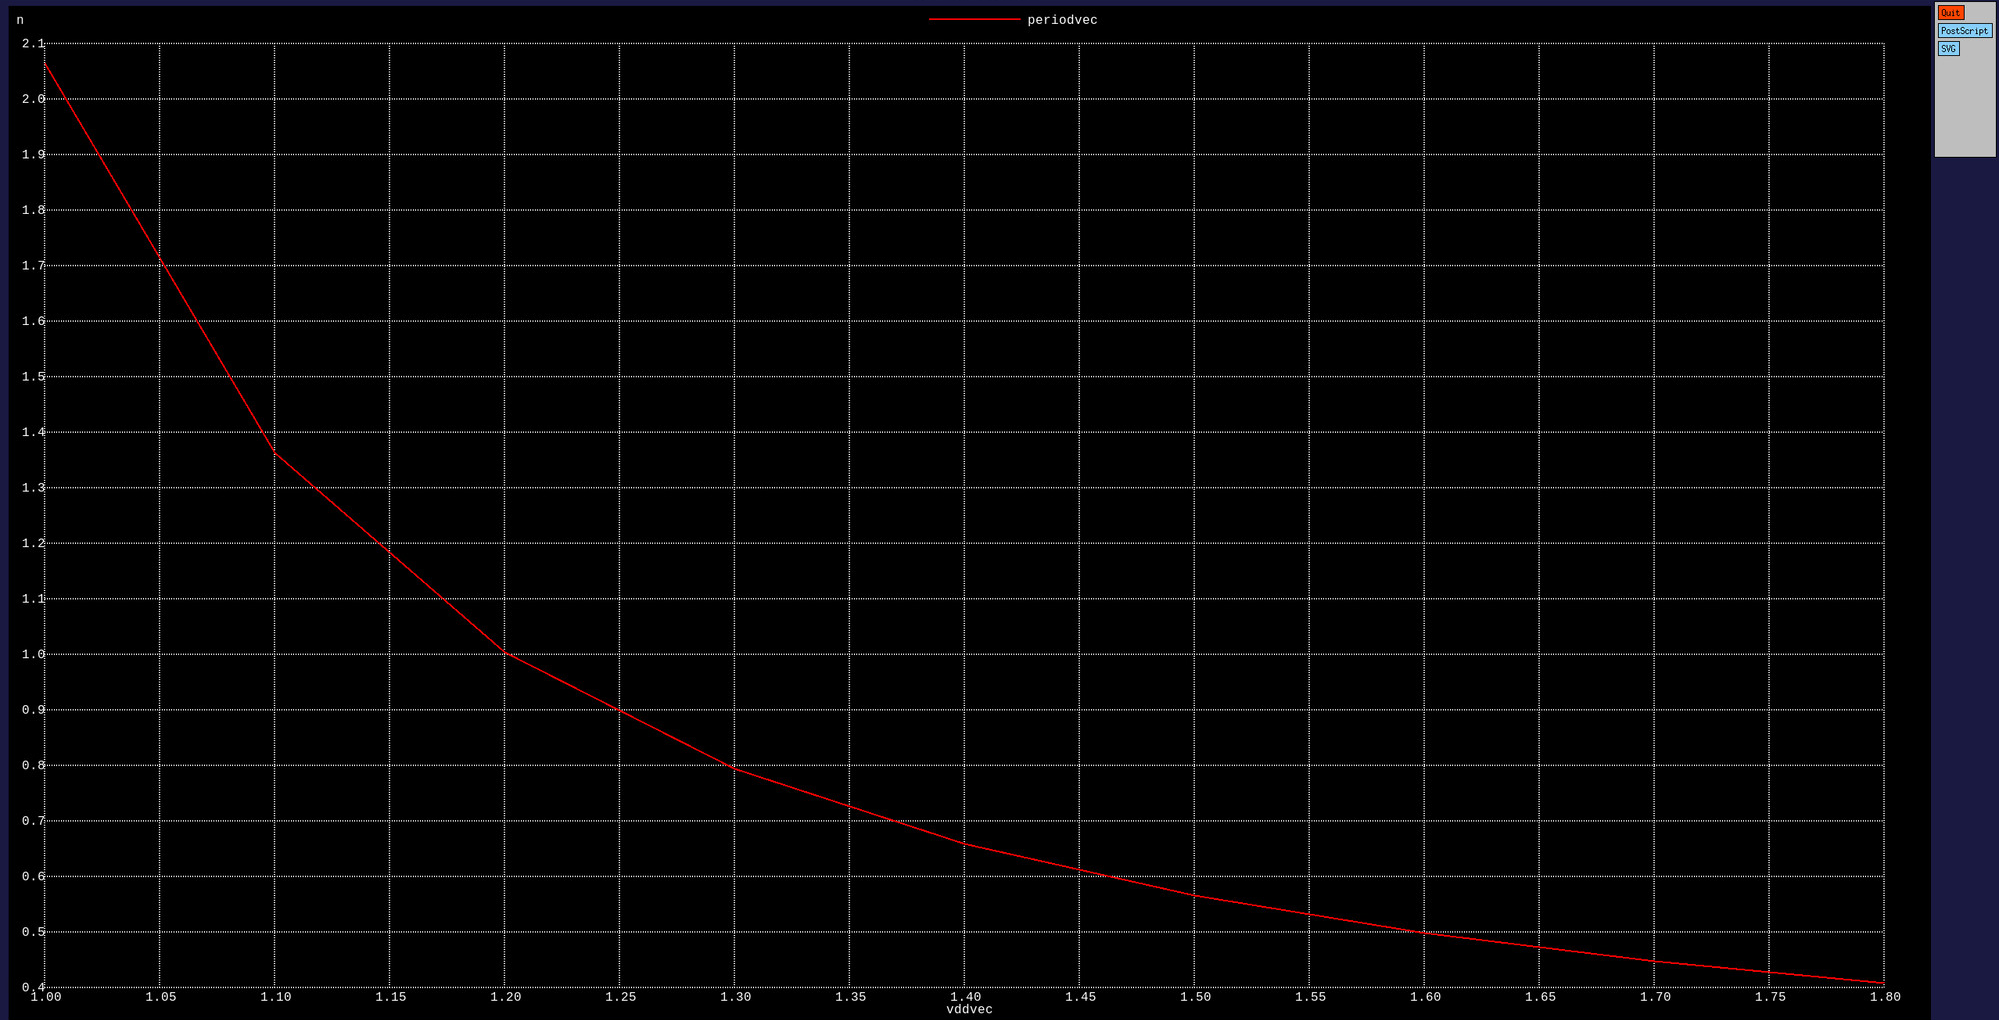
\includegraphics[width=0.85\textwidth]{figures/2b_period.png}
  \caption{Simulated \texttt{periodvec} vs.\ \texttt{vddvec} (7 stages).}
  \label{fig:2b-period}
\end{figure}

\begin{figure}[h]
  \centering
  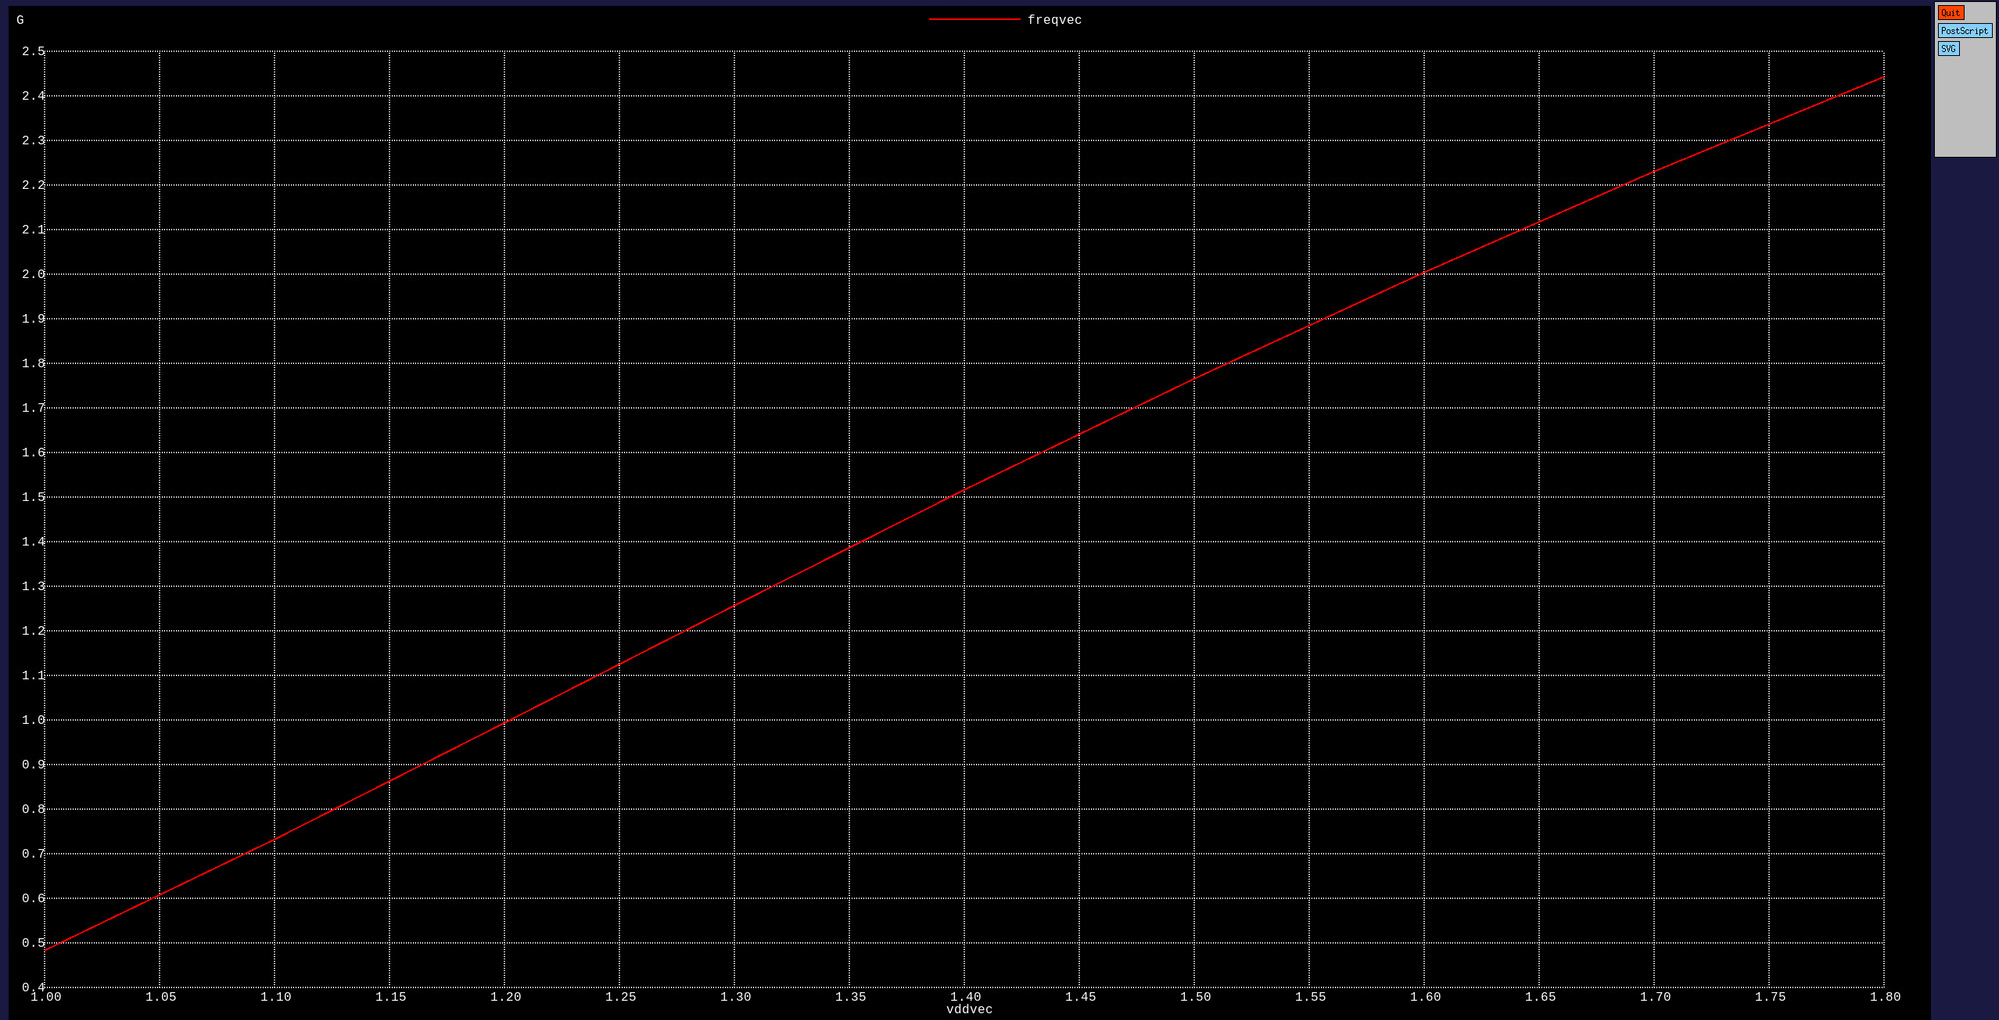
\includegraphics[width=0.85\textwidth]{figures/2b_freq.png}
  \caption{Simulated \texttt{freqvec} vs.\ \texttt{vddvec} (7 stages).}
  \label{fig:2b-freq}
\end{figure}

\begin{table}[h]
  \centering
  \begin{tabular}{|c|c|c|c|c|c|}
    \hline
    $V_{DD}$ (V) & Sim.\ $T$ (ns) & Ana.\ $T$ (ns) & Ratio & Sim.\ $f$ (GHz) & Ana.\ $f$ (GHz) \\
    \hline
    1.0 & 2.07  & 0.799 & 2.59 & 0.483 & 1.251 \\
    1.1 & 1.71  & 0.533 & 3.21 & 0.585 & 1.875 \\
    1.2 & 1.34  & 0.399 & 3.36 & 0.746 & 2.505 \\
    1.3 & 1.00  & 0.321 & 3.12 & 1.000 & 3.120 \\
    1.4 & 0.80  & 0.270 & 2.97 & 1.250 & 3.708 \\
    1.5 & 0.65  & 0.234 & 2.77 & 1.538 & 4.267 \\
    1.6 & 0.545 & 0.209 & 2.61 & 1.835 & 4.794 \\
    1.7 & 0.465 & 0.189 & 2.46 & 2.151 & 5.290 \\
    1.8 & 0.409\textsuperscript{\dag} & 0.174 & 2.35\textsuperscript{\dag} & 2.444\textsuperscript{\dag} & 5.755 \\
    \hline
  \end{tabular}
  \caption{Simulated vs.\ analytical 7-stage ring oscillator period/frequency
  vs.\ $V_{DD}$. All simulated values read off
  Figures~\ref{fig:2b-period}/\ref{fig:2b-freq} except $V_{DD}=1.8$~V
  (\textsuperscript{\dag}), which is the exact Part 2(a) \texttt{meas} value
  ($T=409.12$~ps, $f=2.444$~GHz) and confirms the plot-reading calibration.}
  \label{tab:2b-sim}
\end{table}

\paragraph{Discussion.} As in Part 2(a), the simulated ring is uniformly
slower than the analytical single-stage-delay estimate across the whole
sweep (ratio $>1$ throughout), but the size of that gap is
\textbf{non-monotonic} in $V_{DD}$ -- it grows from $2.6\times$ at
$V_{DD}=1.0$~V to a peak of $\approx3.4\times$ around $V_{DD}=1.2$~V, then
\emph{shrinks} steadily back down to $2.35\times$ at $V_{DD}=1.8$~V (matching
Part 2(a)'s finding exactly, as it should since both come from the same
$V_{DD}=1.8$~V simulation). This differs from Part 1(b)'s single-stage delay
ratio, which grew \emph{monotonically} with $V_{DD}$
(Table~\ref{tab:1b-sim}) -- the ring's steady-state loading effect (each
stage never settling fully between transitions, as seen in
Figure~\ref{fig:2a-waveform}) evidently interacts with $V_{DD}$ differently
than a single isolated FO1 transition does, and is most pronounced at
intermediate $V_{DD}\approx1.2$~V rather than growing monotonically. Both
simulated curves (period and frequency) are smooth and monotonic in $V_{DD}$
themselves (Figures~\ref{fig:2b-period}, \ref{fig:2b-freq}), just uniformly
offset from -- and non-uniformly scaled relative to -- the analytical
prediction.

\subsection{Part (c): Frequency/Period vs.\ $V_{DD}$, $N=9$}

\subsubsection{Calculation}

Applying $f_{osc}=1/(2\,N\,t_p(V_{DD}))$ with $N=9$ (a $9/7\approx1.29\times$
scaling down of every frequency in Table~\ref{tab:2b-analytical}):

\begin{table}[h]
  \centering
  \begin{tabular}{|c|c|c|c|}
    \hline
    $V_{DD}$ (V) & $t_p$ (ps) & $f_{osc}$ (GHz) & $T$ (ps) \\
    \hline
    1.0 & 57.10 & 0.973 & 1027.8 \\
    1.1 & 38.09 & 1.459 & 685.5 \\
    1.2 & 28.51 & 1.948 & 513.2 \\
    1.3 & 22.90 & 2.426 & 412.2 \\
    1.4 & 19.26 & 2.884 & 346.7 \\
    1.5 & 16.74 & 3.319 & 301.3 \\
    1.6 & 14.90 & 3.729 & 268.2 \\
    1.7 & 13.50 & 4.114 & 243.1 \\
    1.8 & 12.41 & 4.476 & 223.4 \\
    \hline
  \end{tabular}
  \caption{Analytical 9-stage ring oscillator frequency/period vs.\ $V_{DD}$.}
  \label{tab:2c-analytical}
\end{table}

\subsubsection{Schematic}

\begin{figure}[h]
  \centering
  
\includegraphics[width=0.95\textwidth]{figures/2c_schematic.png}
  \caption{9-stage ring oscillator (\texttt{assign2c.sch}, \texttt{x1}--\texttt{x9}),
  same per-stage inverter as Figure~\ref{fig:2a-schematic}.}
  \label{fig:2c-schematic}
\end{figure}

\subsubsection{Measurement}

\texttt{assign2c.spice} is identical to \texttt{assign2b.spice} except the
ring is extended to 9 stages (\texttt{x1}--\texttt{x9}) before closing back to
\texttt{vout}; the \texttt{.control} block (sweep, \texttt{meas}, plot) is
unchanged.

\begin{figure}[h]
  \centering
  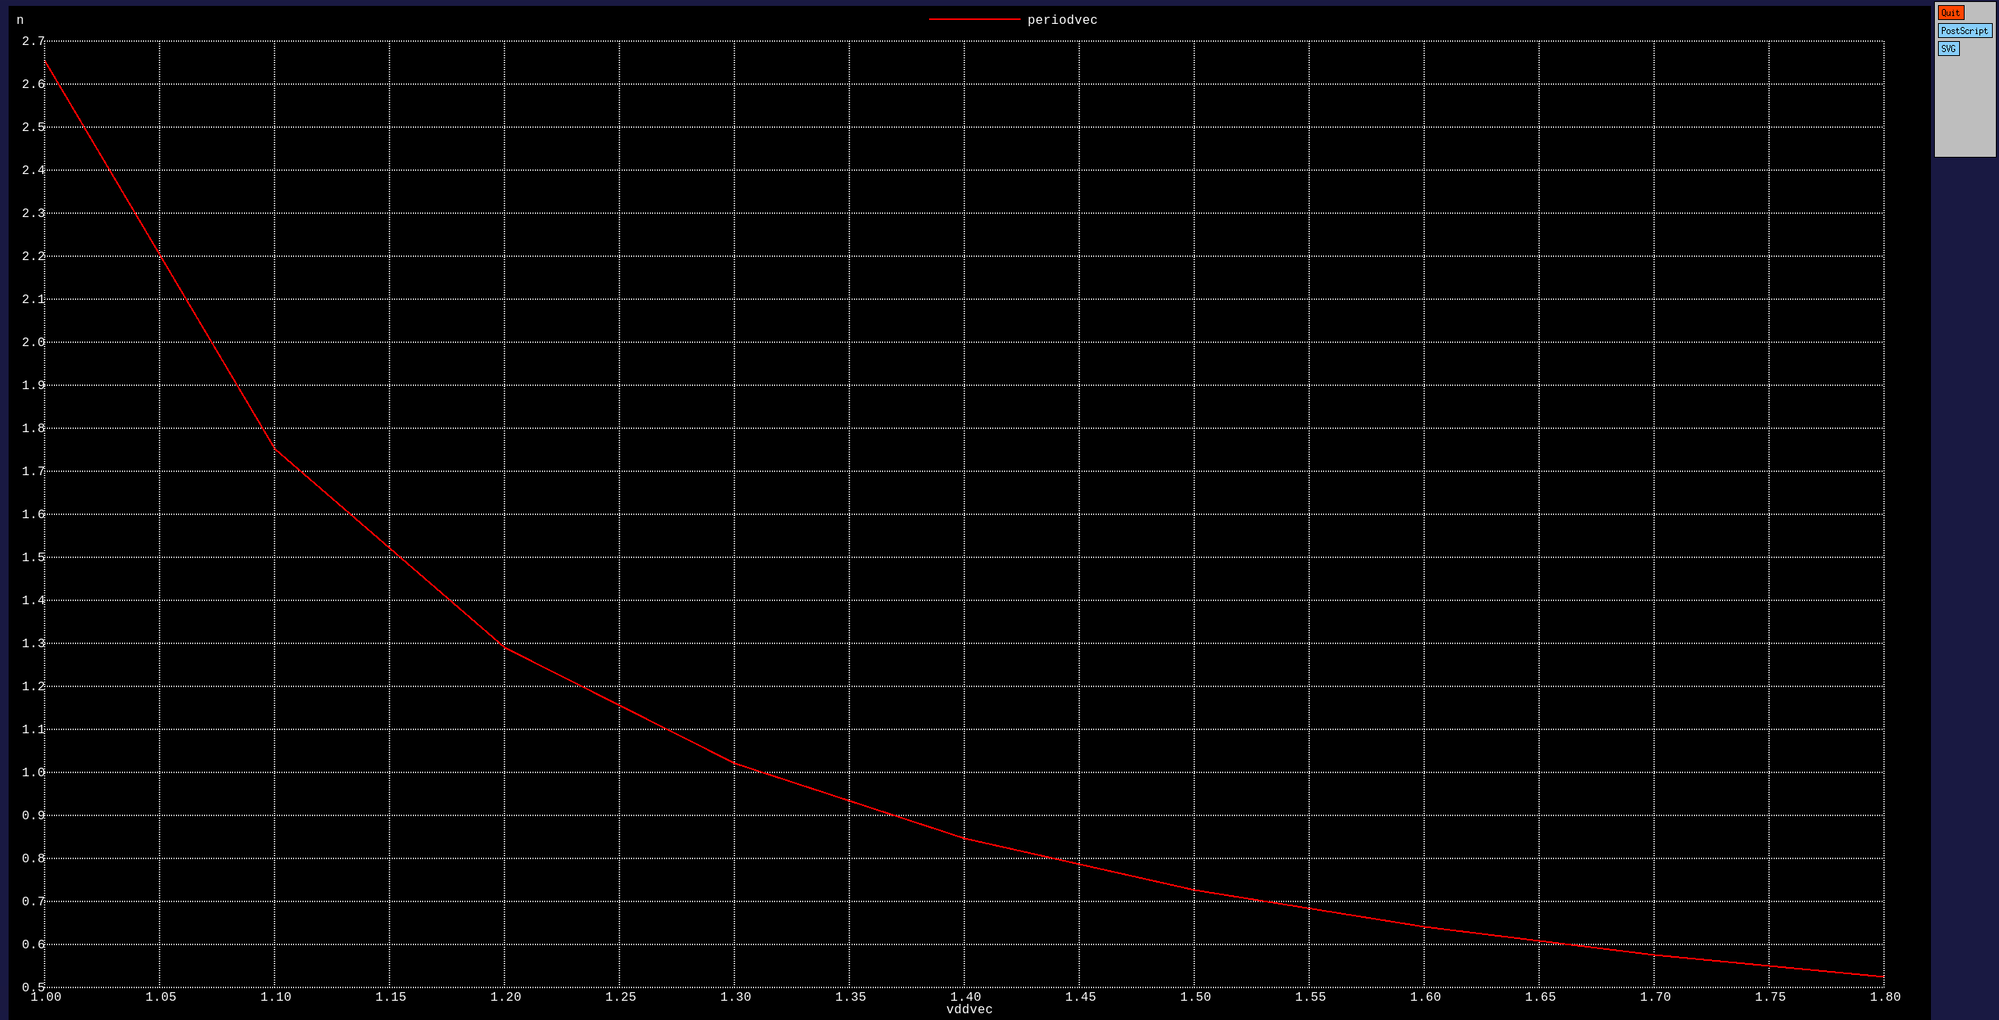
\includegraphics[width=0.85\textwidth]{figures/2c_period.png}
  \caption{Simulated \texttt{periodvec} vs.\ \texttt{vddvec} (9 stages).}
  \label{fig:2c-period}
\end{figure}

\begin{figure}[h]
  \centering
  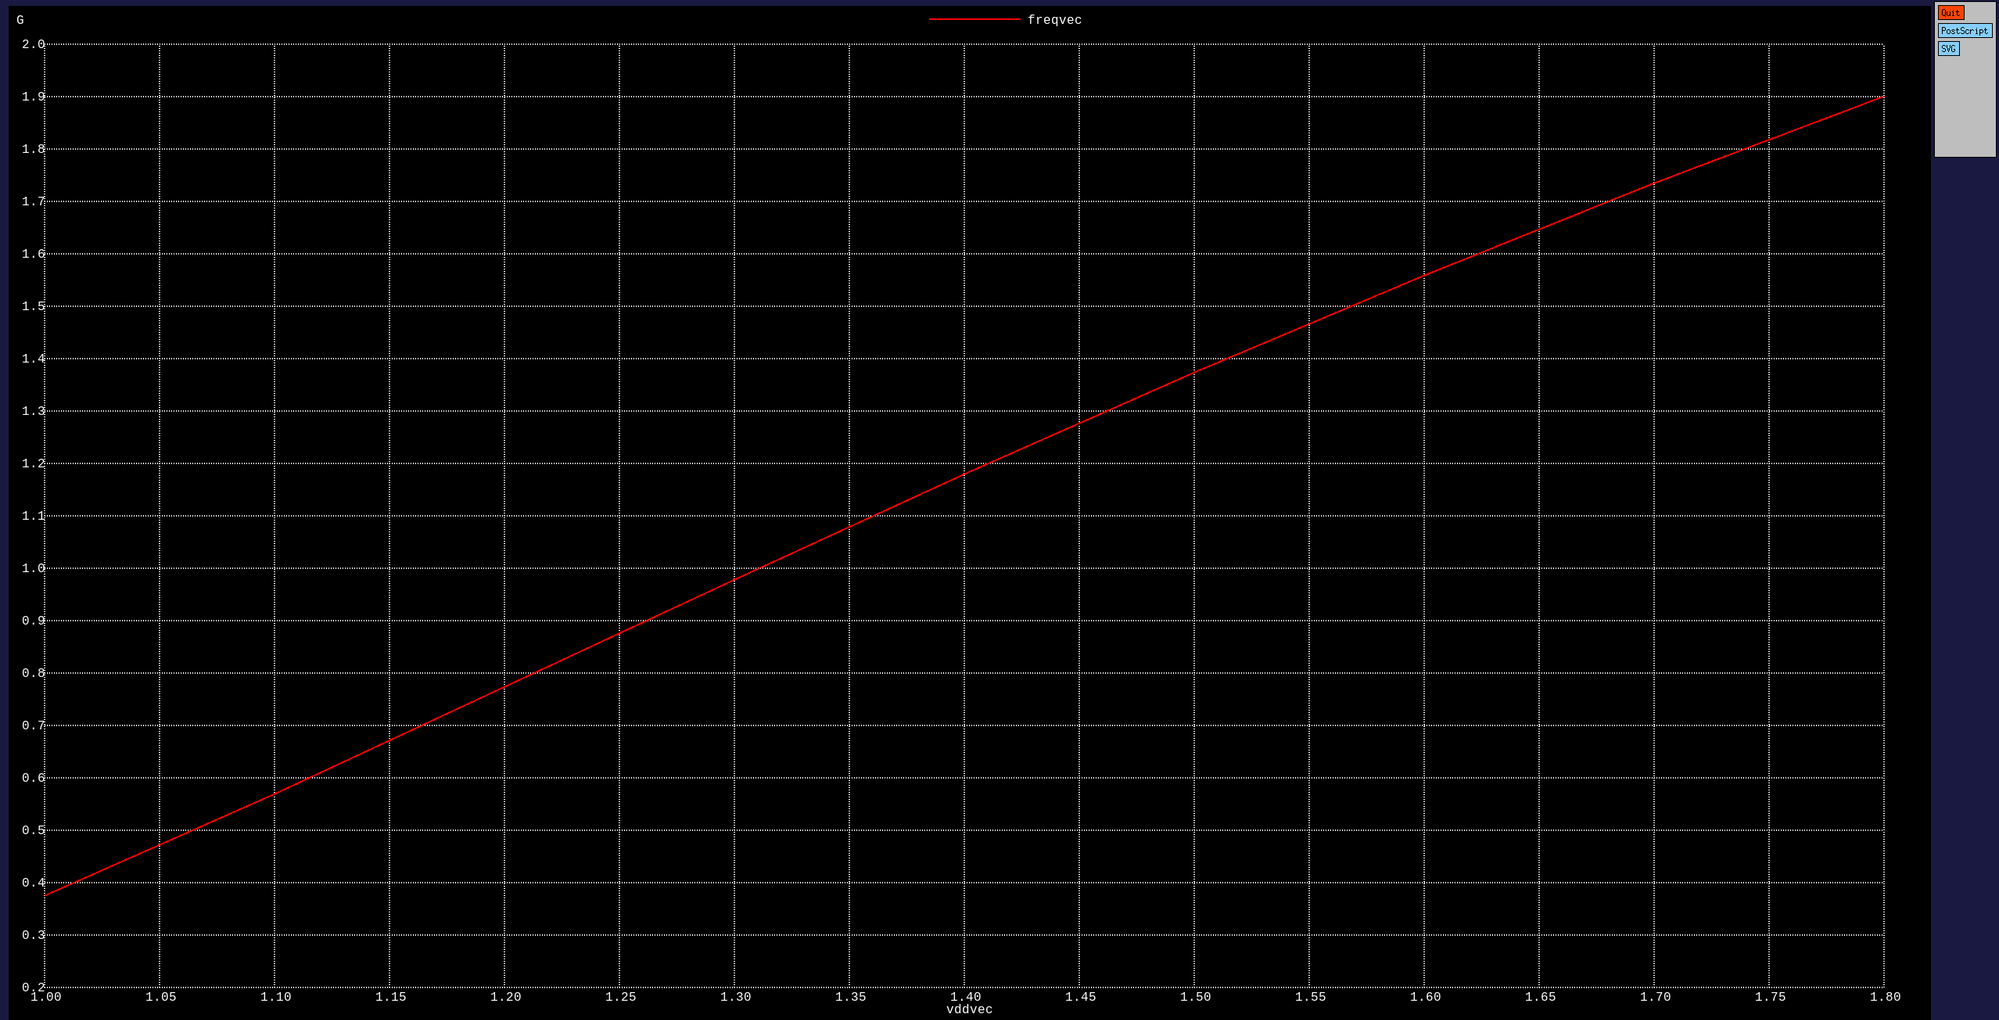
\includegraphics[width=0.85\textwidth]{figures/2c_freq.png}
  \caption{Simulated \texttt{freqvec} vs.\ \texttt{vddvec} (9 stages).}
  \label{fig:2c-freq}
\end{figure}

\begin{table}[h]
  \centering
  \begin{tabular}{|c|c|c|c|c|c|c|}
    \hline
    $V_{DD}$ (V) & Sim.\ $T$ (ns) & Ana.\ $T$ (ns) & Ratio & Sim.\ $f$ (GHz) & Ana.\ $f$ (GHz) & $f_9/f_7$ (sim) \\
    \hline
    1.0 & 2.68  & 1.028 & 2.61 & 0.373 & 0.973 & 0.772 \\
    1.1 & 2.20  & 0.686 & 3.21 & 0.455 & 1.459 & 0.778 \\
    1.2 & 1.75  & 0.513 & 3.41 & 0.571 & 1.948 & 0.766 \\
    1.3 & 1.30  & 0.412 & 3.15 & 0.769 & 2.426 & 0.769 \\
    1.4 & 1.05  & 0.347 & 3.03 & 0.952 & 2.884 & 0.762 \\
    1.5 & 0.85  & 0.301 & 2.82 & 1.176 & 3.319 & 0.765 \\
    1.6 & 0.70  & 0.268 & 2.61 & 1.429 & 3.729 & 0.779 \\
    1.7 & 0.605 & 0.243 & 2.49 & 1.653 & 4.114 & 0.769 \\
    1.8 & 0.526 & 0.223 & 2.36 & 1.901 & 4.476 & 0.778 \\
    \hline
  \end{tabular}
  \caption{Simulated vs.\ analytical 9-stage ring oscillator period/frequency
  vs.\ $V_{DD}$, all read off Figures~\ref{fig:2c-period}/\ref{fig:2c-freq}
  (cross-checked against each other via $T=1/f$, and against the $N=9/N=7$
  scaling argument below). Last column: simulated 9-stage frequency divided
  by the corresponding simulated 7-stage frequency
  (Table~\ref{tab:2b-sim}), compared to the ideal $7/9\approx0.778$
  prediction.}
  \label{tab:2c-sim}
\end{table}

\paragraph{Discussion.} The 9-stage ring reproduces the same qualitative
picture as the 7-stage ring: uniformly slower than the analytical estimate
(ratio $2.4$--$3.4\times$), with the same non-monotonic ratio-vs-$V_{DD}$
shape peaking around $V_{DD}\approx1.2$~V -- as expected, since both rings
share the identical per-stage inverter and the same steady-state loading
mechanism identified in Part (a)/(b).

The more interesting result is the last column of Table~\ref{tab:2c-sim}: the
ratio of simulated $N=9$ to simulated $N=7$ frequency at each $V_{DD}$ comes
out to $0.762$--$0.779$ across the whole sweep, averaging almost exactly the
ideal analytical prediction of $7/9\approx0.778$ (within
$\sim1$--$2\%$ at most points, well within plot-reading precision). In other
words, even though the \emph{absolute} per-stage delay in both rings is
inflated well beyond the single-stage analytical estimate (by the
steady-state loading effect discussed in Part (a)), that inflation is
essentially \textbf{independent of the ring length $N$} -- it does not grow
with the number of stages, so the simple $f_{osc}\propto1/N$ scaling from the
Calculation model still holds almost exactly between the two simulated
rings. This is a cleaner result than the earlier working hypothesis (that
$N$-dependent loading, i.e.\ each stage driving one more identical fan-out
around a longer loop, might explain part of the analytical gap): the data
shows no such $N$-dependence, so the entire gap from Table~\ref{tab:2b-sim}/
\ref{tab:2c-sim} must instead come from the ring's steady-state (never fully
settling) switching behavior itself, common to any $N$, rather than from
loop length.
